\documentclass[12pt,a4paper]{article}

% --- Настройка языка и шрифтов для LuaLaTeX ---
\usepackage{fontspec}
\defaultfontfeatures{Ligatures=TeX,Scale=MatchLowercase}

\setmainfont{Alice-Regular}[
    Path=font/,
    Extension=.ttf,
    BoldFont = Alice-Regular,
    ItalicFont = Alice-Regular,
    BoldItalicFont = Alice-Regular,
    BoldFeatures = {FakeBold=1.6},
    ItalicFeatures = {FakeSlant=0.2},
    BoldItalicFeatures = {FakeBold=1.6,FakeSlant=0.2}
]

\newfontfamily\cyrillicfont{Alice-Regular}[
    Path=font/,
    Extension=.ttf,
    BoldFont = Alice-Regular,
    ItalicFont = Alice-Regular,
    BoldItalicFont = Alice-Regular,
    BoldFeatures = {FakeBold=1.6},
    ItalicFeatures = {FakeSlant=0.2},
    BoldItalicFeatures = {FakeBold=1.6,FakeSlant=0.2}
]

\usepackage{polyglossia}
\setmainlanguage{russian}
\setsansfont{TeX Gyre Heros}
\setmonofont{TeX Gyre Cursor}

\usepackage{graphicx}        					          % Графика
\usepackage[protrusion=false]{microtype}       	% Микротипографика
\usepackage{amsmath, amsfonts, amssymb, amsthm}	% Математика
\usepackage{braket} 							              % Braket нотация для квантовой механики
\usepackage{unicode-math} 						          % Современный пакет для математики в LuaLaTeX
\usepackage{longtable}       					          % Таблицы с разрывом страниц
\usepackage{tikz}           					          % Рисование
\usepackage[europeanresistors]{circuitikz}		  % Рисование электрических схем в европейском стиле
\usepackage{listings}                              % Для отображения кода
\usepackage{listingsutf8}                          % Поддержка UTF-8 в listings
\usepackage{tabularx}       					          % Для таблиц во всю ширину
\usepackage{array}		  						            % Для расширенных возможностей таблиц
\usepackage{float}          					          % Для точного позиционирования фигур
\usepackage{pgfplots}                           % Для построения графиков
\usepackage{caption}                            % Для настройки подписей к рисункам и таблицам
\usepackage{xfp}                                % Для вычислений в LaTeX
\usepackage{luacode}                            % Для выполнения Lua-кода в документе    
\pgfplotsset{compat=1.18}
\usepackage[a4paper,left=20mm,right=20mm,top=20mm,bottom=20mm]{geometry}

\usetikzlibrary{arrows.meta}

% --- Колонтитулы ---
\usepackage{fancyhdr}
\pagestyle{fancy}
\fancyhf{}

\renewcommand{\headrulewidth}{0.4pt}
\renewcommand{\footrulewidth}{0.4pt}
\renewcommand\lstlistingname{Исходный код}

\lstdefinestyle{main}{
    backgroundcolor=\color{gray!8},
    commentstyle=\color{green!50!black},
    keywordstyle=\color{blue!80!black},
    numberstyle=\small\color{darkgray},
    stringstyle=\rmfamily\color{orange!90!black},
    basicstyle=\ttfamily\small,
    columns=fixed,
    extendedchars=true,
    inputencoding=utf8,
    breakatwhitespace=false,
    breaklines=true,
    keepspaces=true,
    numbers=left,
    numbersep=8pt,
    showspaces=false,
    showstringspaces=false,
    showtabs=false,
    tabsize=4
}

\lstset{style=main}

\newcolumntype{C}{>{\centering\arraybackslash}X}
\renewcommand{\arraystretch}{1.25}

% =========================================================
%         СЛУЖЕБНЫЕ КОМАНДЫ ДЛЯ ВЫЧИСЛЕНИЙ
% =========================================================
\newcommand{\CalcZero} [1]{\fpeval{round((#1),0)}}
\newcommand{\CalcOne}  [1]{\fpeval{round((#1),1)}}
\newcommand{\CalcTwo}  [1]{\fpeval{round((#1),2)}}
\newcommand{\CalcThree}[1]{\fpeval{round((#1),3)}}
\newcommand{\CalcFour} [1]{\fpeval{round((#1),4)}}
\newcommand{\CalcFive} [1]{\fpeval{round((#1),5)}}

\begin{luacode*}
-- безопасная версия value_with_mantice
local function round_fallback(x)
  if x >= 0 then return math.floor(x + 0.5) else return math.ceil(x - 0.5) end
end
local round = math.round or round_fallback

function value_with_mantice(value, precision, shift, scale)
  precision = precision or 5
  shift = shift or 0
  scale = scale or 0

  if value == nil or value ~= value then
    return "\\fpeval{0}"
  end
  if value == 0 then
    return "\\fpeval{0}"
  end

  local sign = ""
  if value < 0 then
    sign = "-"
    value = math.abs(value)
  end

  local logv = math.log10(value)
  if not (logv == logv) then -- проверка на NaN
    return "\\fpeval{0}"
  end

  local floorlog = math.floor(logv)
  local mantissa = round(value * 10^(precision - 1 - floorlog)) * 10^(-(precision - 1) + shift - scale)
  local exponent = floorlog - shift

  if exponent == 0 then
    return sign .. "\\fpeval{" .. mantissa .. "}"
  else
    return sign .. "\\fpeval{" .. mantissa .. "} \\cdot 10^{" .. exponent .. "}"
  end
end



\end{luacode*}

% ---------------------------------------------------------
% ОБЩИЕ ДАННЫЕ
% ---------------------------------------------------------
\def\VariantN{1}          					         % Номер варианта
\def\StudentName{Андреев Иван Алексеевич}  	 % ФИО студента
\def\TeacherName{Терещенко Анатолий Михайлович} % ФИО преподавателя
\def\LabNumber{7}							               % Номер лабораторной работы
\def\Discipline{Численные методы}				           % Название дисциплины
\def\LabTitle{Конечноразностные методы решения дифференциальных уравнений}	 % Название лабораторной работы

\title{
	МИНОБРНАУКИ РОССИИ

	федеральное государственное автономное образовательное учреждение

	высшего образования

	«Национальный исследовательский университет
	«Московский институт электронной техники»
	\vspace{2em}
}
\author{
}
\date{}

\begin{document}

\maketitle
\thispagestyle{fancy}

\begin{center}
\Large Отчёт по Лабораторной работе $\LabNumber$\\
по дисциплине «\Discipline»\\
«\LabTitle»
\end{center}

\begin{center}
\Large Вариант \VariantN
\end{center}

\vspace{12em}

\begin{table}[h]
\noindent
\begin{tabular*}{\textwidth}{@{\extracolsep{\fill}} p{0.48\textwidth} p{0.52\textwidth}}
Студент, группа & \StudentName, ЭН-$25$ \\
[0.5em] Руководитель & \TeacherName
\end{tabular*}
\end{table}

\cfoot{Москва 2026}

\pagebreak

\fancyhead[L]{\LabTitle} 
\fancyhead[R]{\Discipline}
\fancyfoot[C]{\thepage}

\fancyhead[L]{Теория}
\fancyhead[R]{\LabTitle}

\begin{center}
\Large\textbf{Лабораторная работа $\LabNumber$}
\end{center}

\begin{center}
\LARGE\textbf{\LabTitle}
\end{center}

\large\textbf{\textit{Цель работы}:} Изучение задачи численного решения краевых задач для ОДУ 2-го
порядка. Изучение методов решения СЛАУ методом прогонки. Приобретение навыков программирования методов численного решения
ОДУ.

\section{Теоретические сведения}

\subsection{Метод прогонки}

Рассмотрим краевую задачу для обыкновенного дифференциального уравнения второго порядка
\begin{equation*}
    y''(x) + p(x)y'(x) + q(x)y(x) = f(x), \qquad x \in [a,b],
\end{equation*}
с краевыми условиями общего вида
\begin{equation*}
    k_1 y(a) + k_2 y'(a) = \alpha, \qquad
    k_3 y(b) + k_4 y'(b) = \beta.
\end{equation*}

Для численного решения вводится равномерная сетка
\begin{equation*}
    x_i = a + ih, \qquad i = 0,1,\ldots,n, \qquad
    h = \frac{b-a}{n}.
\end{equation*}

Сеточное значение искомой функции в узле $x_i$ обозначим как
\begin{equation*}
    y_i \approx y(x_i).
\end{equation*}

Внутри отрезка, то есть при $i = 1,2,\ldots,n-1$, производные аппроксимируются центральными разностями
\begin{equation*}
    y'(x_i) \approx \frac{y_{i+1}-y_{i-1}}{2h},
    \qquad
    y''(x_i) \approx \frac{y_{i+1}-2y_i+y_{i-1}}{h^2}.
\end{equation*}

Тогда разностный аналог исходного дифференциального уравнения имеет вид
\begin{equation*}
    \frac{y_{i+1}-2y_i+y_{i-1}}{h^2}
    +
    p_i \frac{y_{i+1}-y_{i-1}}{2h}
    +
    q_i y_i
    =
    f_i,
\end{equation*}
где
\begin{equation*}
    p_i = p(x_i), \qquad q_i = q(x_i), \qquad f_i = f(x_i).
\end{equation*}

После группировки коэффициентов при $y_{i-1}$, $y_i$, $y_{i+1}$ получаем трёхдиагональную систему
\begin{equation*}
    a_i y_{i-1} + b_i y_i + c_i y_{i+1} = f_i,
    \qquad i = 1,2,\ldots,n-1,
\end{equation*}
где
\begin{equation*}
    a_i = \frac{1}{h^2} - \frac{p_i}{2h},
    \qquad
    b_i = q_i - \frac{2}{h^2},
    \qquad
    c_i = \frac{1}{h^2} + \frac{p_i}{2h}.
\end{equation*}

Краевые условия также необходимо привести к виду, совместимому с трёхдиагональной системой. Если используются условия общего вида
\begin{equation*}
    k_1 y(a) + k_2 y'(a) = \alpha,
    \qquad
    k_3 y(b) + k_4 y'(b) = \beta,
\end{equation*}
то при аппроксимации первой производной с первым порядком точности получаем
\begin{equation*}
    y'(a) \approx \frac{y_1-y_0}{h},
    \qquad
    y'(b) \approx \frac{y_n-y_{n-1}}{h}.
\end{equation*}

Отсюда коэффициенты первого и последнего уравнений системы принимают вид
\begin{equation*}
    b_0 = k_1 - \frac{k_2}{h},
    \qquad
    c_0 = \frac{k_2}{h},
    \qquad
    f_0 = \alpha,
\end{equation*}
\begin{equation*}
    a_n = -\frac{k_4}{h},
    \qquad
    b_n = k_3 + \frac{k_4}{h},
    \qquad
    f_n = \beta.
\end{equation*}

Таким образом, вся система линейных алгебраических уравнений имеет вид
\begin{equation*}
\begin{cases}
    b_0 y_0 + c_0 y_1 = f_0, \\[4pt]
    a_i y_{i-1} + b_i y_i + c_i y_{i+1} = f_i,
    \qquad i = 1,2,\ldots,n-1, \\[4pt]
    a_n y_{n-1} + b_n y_n = f_n.
\end{cases}
\end{equation*}

Если краевые условия заданы непосредственно через значения функции, например
\begin{equation*}
    y(a) = A, \qquad y(b) = B,
\end{equation*}
то соответствующие коэффициенты задаются проще:
\begin{equation*}
    b_0 = 1, \qquad c_0 = 0, \qquad f_0 = A,
\end{equation*}
\begin{equation*}
    a_n = 0, \qquad b_n = 1, \qquad f_n = B.
\end{equation*}

Полученная система имеет трёхдиагональную матрицу:
\begin{equation*}
\begin{pmatrix}
b_0 & c_0 & 0 & \cdots & 0 \\
a_1 & b_1 & c_1 & \cdots & 0 \\
0 & a_2 & b_2 & \cdots & 0 \\
\vdots & \vdots & \vdots & \ddots & c_{n-1} \\
0 & 0 & 0 & a_n & b_n
\end{pmatrix}
\begin{pmatrix}
y_0 \\ y_1 \\ y_2 \\ \vdots \\ y_n
\end{pmatrix}
=
\begin{pmatrix}
f_0 \\ f_1 \\ f_2 \\ \vdots \\ f_n
\end{pmatrix}.
\end{equation*}

Для решения такой системы используется метод прогонки. Идея метода заключается в том, что неизвестные выражаются в виде
\begin{equation*}
    y_i = \alpha_i y_{i+1} + \beta_i,
    \qquad i = 0,1,\ldots,n-1.
\end{equation*}

Из первого уравнения системы
\begin{equation*}
    b_0 y_0 + c_0 y_1 = f_0
\end{equation*}
получаем начальные прогоночные коэффициенты
\begin{equation*}
    \alpha_0 = -\frac{c_0}{b_0},
    \qquad
    \beta_0 = \frac{f_0}{b_0}.
\end{equation*}

Для последующих строк системы вводится обозначение
\begin{equation*}
    d_i = a_i \alpha_{i-1} + b_i.
\end{equation*}

Тогда коэффициенты прямой прогонки при $i = 1,2,\ldots,n-1$ вычисляются по формулам
\begin{equation*}
    \alpha_i = -\frac{c_i}{d_i},
    \qquad
    \beta_i = \frac{f_i - a_i \beta_{i-1}}{d_i}.
\end{equation*}

Последнее значение $y_n$ находится из последнего уравнения системы:
\begin{equation*}
    y_n =
    \frac{f_n - a_n \beta_{n-1}}
    {a_n \alpha_{n-1} + b_n}.
\end{equation*}

После этого выполняется обратная прогонка:
\begin{equation*}
    y_i = \alpha_i y_{i+1} + \beta_i,
    \qquad i = n-1,n-2,\ldots,0.
\end{equation*}

Таким образом, алгоритм метода прогонки состоит из двух этапов:
\begin{enumerate}
    \item Прямая прогонка: вычисляются коэффициенты $\alpha_i$ и $\beta_i$.
    \item Обратная прогонка: последовательно находятся значения $y_i$ от правого конца сетки к левому.
\end{enumerate}

Для корректной работы метода необходимо, чтобы знаменатели в формулах прямой прогонки не обращались в ноль:
\begin{equation*}
    d_i = a_i \alpha_{i-1} + b_i \neq 0,
    \qquad i = 1,2,\ldots,n.
\end{equation*}

На практике это условие проверяется как
\begin{equation*}
    |d_i| > \varepsilon,
\end{equation*}
где $\varepsilon$ --- достаточно малое положительное число, например $10^{-12}$.

Метод прогонки считается устойчивым, если прогоночные коэффициенты не приводят к быстрому накоплению погрешности округления. В лабораторной работе для проверки устойчивости используется условие
\begin{equation*}
    |\alpha_i| < 1,
    \qquad i = 0,1,\ldots,n-1.
\end{equation*}

\section{Реализация метода прогонки}

Код программы, с помощью параметров $p$, $q$ и $f$ реализована сама функция, с помощью
$a(1)$, $b(1)$, $c(1)$, $d(1)$ и $a(N)$, $b(N)$, $c(N)$, $d(N)$ задаются краевые условия. 
\begin{equation*}
    y''(x) - (x + 1)y'(x) - y(x) = \frac{2}{(x + 1)^3}
    \qquad x \in [0, 1] \quad y(0) = 1 \quad y(1) = 0.5
\end{equation*}

\begin{lstlisting}[language=Matlab, firstnumber=1, 
	title={\textbf{lab7nm.m}}, escapeinside={(*@}{@*)}]
clear; clc; close all;                    

n = 50;                                    
x0 = 0;                                    
xn = 1;                                    
h = (xn - x0) / n;                         
x = x0:h:xn;                               

% Variant 1
p = @(x) -(x + 1);                     
q = @(x) -1;                  
f = @(x) 2 / (x + 1)^3;                       

N = n + 1;                              

a = zeros(1, N);                           
b = zeros(1, N);                           
c = zeros(1, N);                           
d = zeros(1, N);                           

for i = 2:n                                
    xi = x(i);                             

    a(i) = 1/h^2 - p(xi)/(2*h);            
    b(i) = q(xi) - 2/h^2;                  
    c(i) = 1/h^2 + p(xi)/(2*h);            
    d(i) = f(xi);                          
end                            

% Left boundary condition y(0) = 1
a(1) = 0;
b(1) = 1;
c(1) = 0;
d(1) = 1;

% Right boundary condition y(1) = 0.5
a(N) = 0;
b(N) = 1;
c(N) = 0;
d(N) = 0.5;                              

A = zeros(N, N);    

A(1,1) = b(1);                             
A(1,2) = c(1);                             

for i = 2:n                                
    A(i,i-1) = a(i);                       
    A(i,i) = b(i);                         
    A(i,i+1) = c(i);                       
end

A(N,N-1) = a(N);                           
A(N,N) = b(N);                             

P = zeros(1, N);       
Q = zeros(1, N);       

P(1) = -c(1) / b(1);                    
Q(1) = d(1) / b(1);                     

u = 1;                         % variable for checking stability

for i = 2:N-1                  % forward sweep
    znam = a(i)*P(i-1) + b(i); % denominator in the sweep formulas

    if abs(znam) < 1e-12               
        u = 0;                             
    end

    P(i) = -c(i) / znam;                   
    Q(i) = (d(i) - a(i)*Q(i-1)) / znam;    
end

znam = a(N)*P(N-1) + b(N);              

if abs(znam) < 1e-12                  
    u = 0;                                 
end

y = zeros(1, N);                 

y(N) = (d(N) - a(N)*Q(N-1)) / znam;        

for i = N-1:-1:1                          
    y(i) = P(i)*y(i+1) + Q(i);           
end

r = A*y' - d';         % Residual of the system for the Thomas algorithm           
norm_r = norm(r);                         

cond_A = cond(A);      % Condition number of the matrix

left_bc = y(1) - 1;    % Check left boundary condition
right_bc = y(N) - 0.5; % Check right boundary condition                          

disp('Residual norm:');
disp(norm_r);                                   

disp('Condition number of matrix A:');  
disp(cond_A);

disp('Left boundary condition residual:');  
disp(left_bc);                             

disp('Right boundary condition residual:'); 
disp(right_bc);                            

if u == 1 && max(abs(P)) < 1   % stability check for the sweep
    disp('Algorithm is stable');       
else
    disp('Algorithm may be unstable'); 
end

figure;                                    
plot(x, y, 'b-o');                          
grid on;                                   
xlabel('x');                               
ylabel('y');                               
title('Solution of the boundary-value problem');
legend('Iteration algorithm');
\end{lstlisting}

\section{Результат работы программы}

\begin{figure}[H]
    \centering
    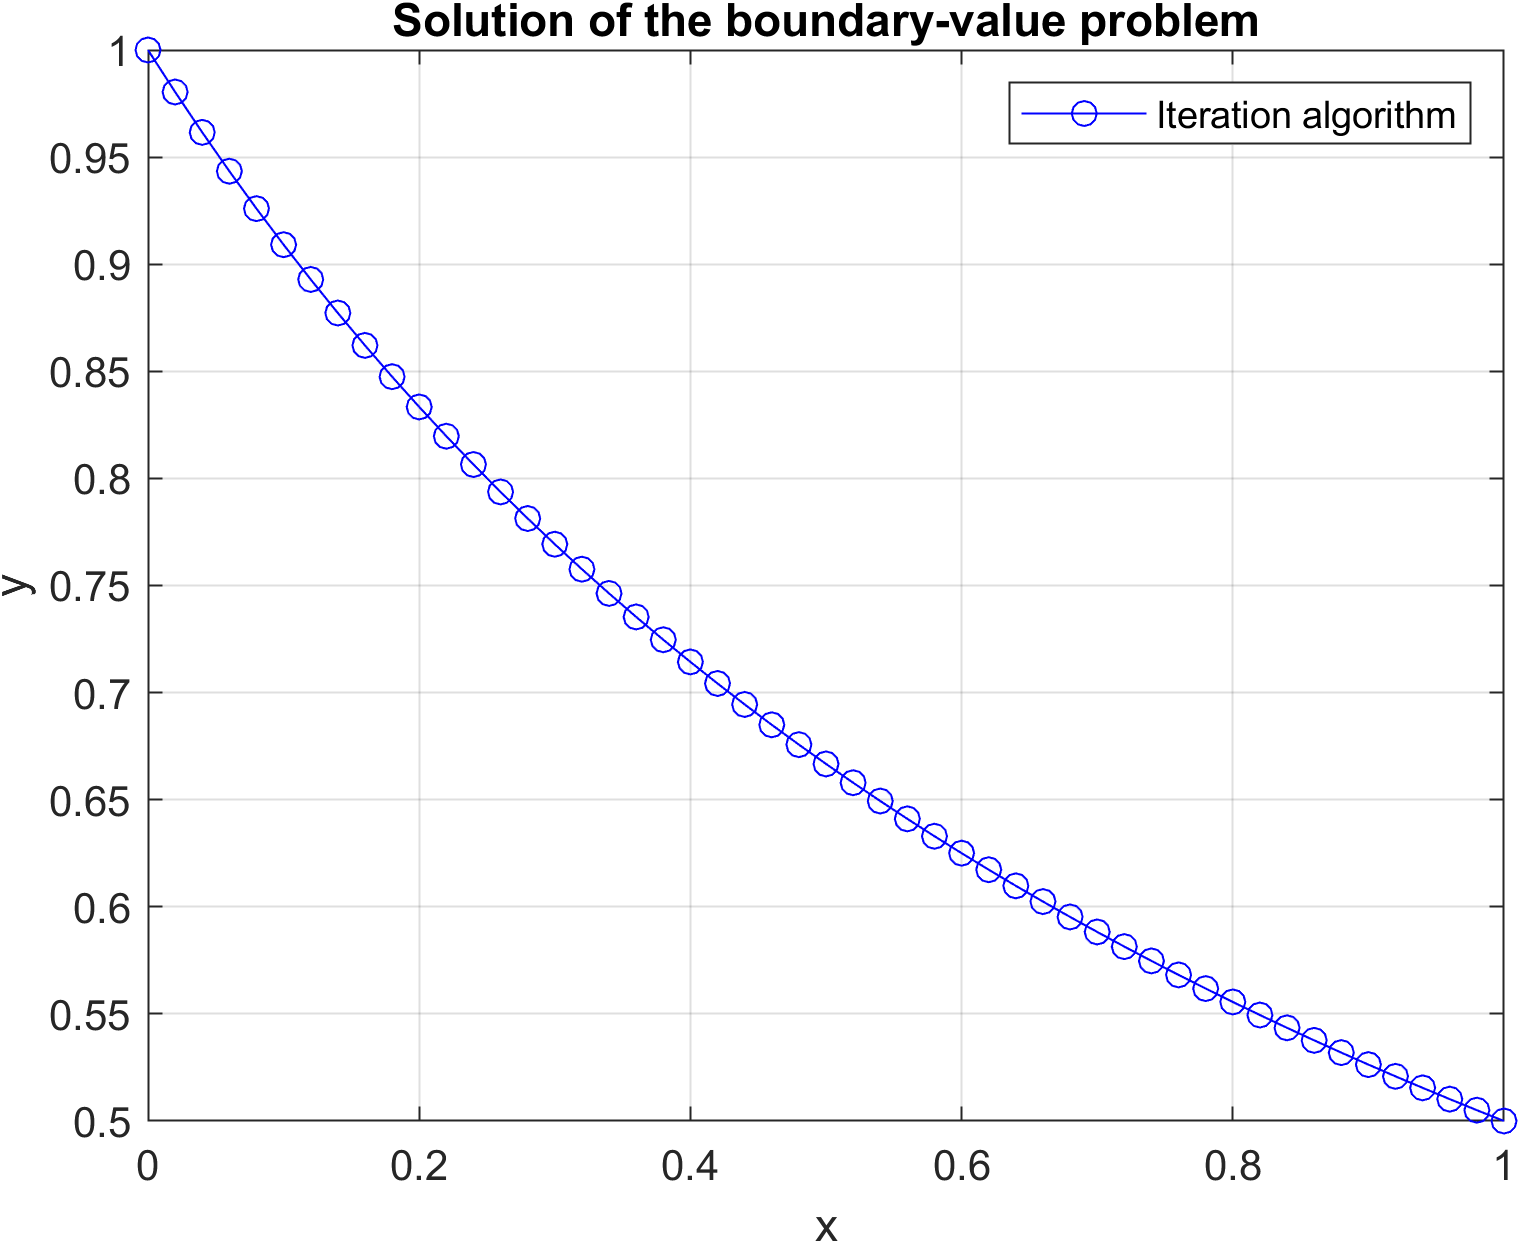
\includegraphics[width=\textwidth]{image1.png}
    \caption{График решения краевой задачи, полученного методом прогонки.}
\end{figure}

Вывод консоли программы:
\begin{verbatim}
Residual norm:
   2.1162e-12

Condition number of matrix A:
   4.8626e+04

Left boundary condition residual:
     0

Right boundary condition residual:
     0

Algorithm is stable
\end{verbatim}

\section{Вывод}

С помощью метода прогонки была успешно решена краевая задача для обыкновенного 
дифференциального уравнения второго порядка. Полученное численное решение соответствует
заданным краевым условиям, что подтверждается нулевыми остатками при проверке граничных
условий. Невысокое значение нормы невязки указывает на высокую точность решения. 
Условие устойчивости метода прогонки выполнено, что гарантирует отсутствие накопления
погрешности при вычислениях. График решения демонстрирует ожидаемое поведение функции
на отрезке заданном отрезке.

\end{document}